\chapter{Implementation of Demonstrations}\label{chp-demonstrations}



\section{NeOn Toolkit Plugin Implementation}
This section describes the NeOn Toolkit the Replica Framework NeOn Toolkit
plugin implementation and presents screenshots of the plugin.

\subsection{NeOn Toolkit Platform}
\index{NeOn Toolkit}
\begin{wrapfigure}{r}{0.5\textwidth}
        \caption{NeOn Toolkit editor GUI}
        \begin{center}
                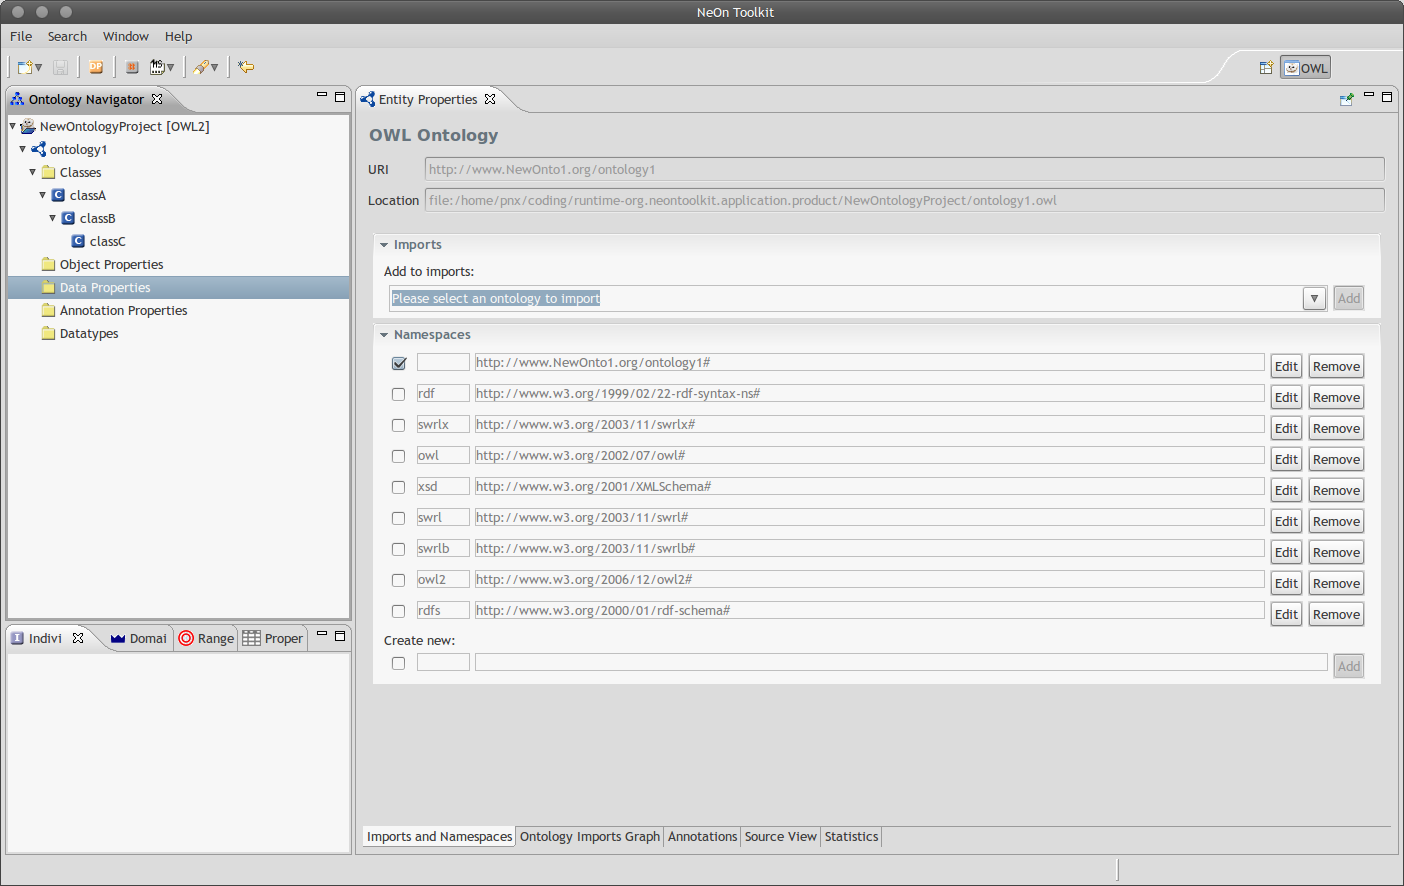
\includegraphics[width=0.5\textwidth]{BilderFrontendImpl/editor.png}
        \end{center}
        \label{fig_editor}
\end{wrapfigure}
The NeOn Toolkit is an ontology engeneering environment implemented as
a desktop application built on the code-base of \index{OntoStudio}
OntoStudio\footnote{OntoStudio is a commerical engineering environment of 
ontoprise, \url{http://www.ontoprise.de/}}, which is in turn based on the
popular IDE Eclipse\index{Eclipse}. The application is implemented as an
Eclipse application with the advantage that the application uses the proven
Eclipse application model and tools of the Eclipse platform.
Technically an Eclipse application is a special plugin which is started
by the eclipse platform. In contrast to usual plugins the lazy-loading
principle does not apply to it and menus and toolbars can be customized
programmatically.

Apart from basic ontology creation the NeOn Toolkit features many other
ontology engineering tools that support in the ontology development lifecycle.

\subsection{Plugin Implementation}
\index{NeOn Toolkit}
The NeOn Toolkit is implemented as an \index{Eclipse}Eclipse\footnote{Eclipse a popular
free, open source \index{IDE}IDE \url{http://www.eclipse.org/}} application. Like
the IDE the application architecture relies on the \index{OSGi}OSGi module system and
service platform\footnote{The Eclipse development community therefore also provides an
implementation of the OSGi specification call Equinox \url{http://www.eclipse.org/equinox/}.}.
Thus the NeOn Toolkit plugin was implemented as an OSGi bundle containing
the necessary meta information required to integrate in the Eclipse
application system.

In addition to the main plugin the NeOn Toolkit bundle containing
the \index{OWLAPI}OWLAPI library had to be modified because the current Replica Framework
implementation requires a patched version.

The plugin integrates smoothly into \index{NeOn Toolkit}NeOn Toolkit and extends its functionality
by adding a Replica Framework project creation wizard and a wizard for
creating shared ontologies as shown in figure \ref{fig_sharedontowizard}.
%\begin{figure}[h]
%       \caption{Replica Framework project creation wizard}
%       \begin{center}
%               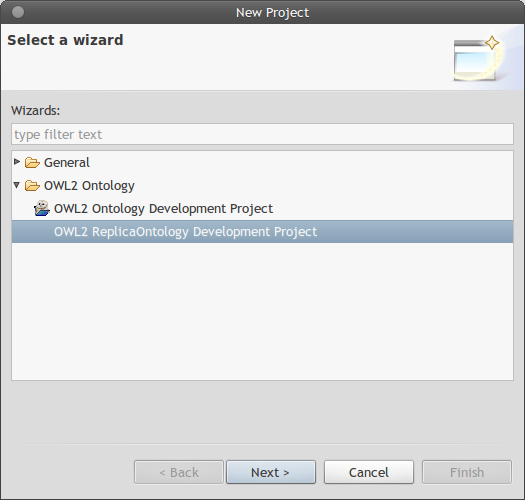
\includegraphics[width=\textwidth/2]{BilderFrontendImpl/wizard0.png}
%       \end{center}
%       \label{img_sharedontowizard0}
%\end{figure}\\
The shared ontology creation wizard also takes care of starting a local Replica Framework server and
initializing an empty shared ontology.

When a shared ontology has been created within a Replica Framework project
the NeOn Toolkit editor shown in figure \ref{fig_editor} can be used to modify
the ontology. All changes
of the ontology are then synchronized with all other connected editors which
enables simultaneous team based development.
\begin{figure}[h]
        \caption{Shared ontology creation wizard}
        \centering
                        \subfloat[Shared ontology project creation wizard.]{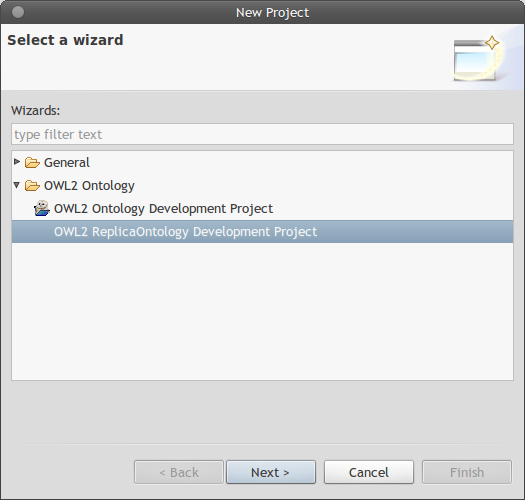
\includegraphics[width=0.45\textwidth]{BilderFrontendImpl/wizard0.png}}
                        \hspace{1cm}
                        \subfloat[Shared ontology project creation wizard.]{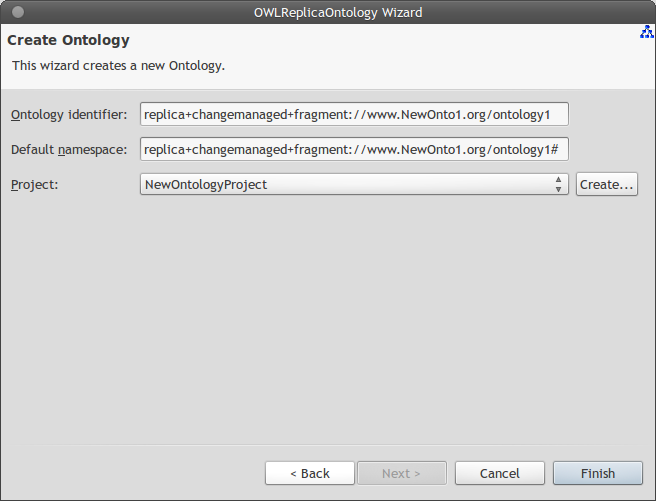
\includegraphics[width=0.45\textwidth]{BilderFrontendImpl/wizard1.png}}
        \label{fig_sharedontowizard}
\end{figure}


\newpage


\section{Replica Framework demonstrator}
\index{JUNG}
\label{replicademonstrator}
The Replica Framework demonstrator is a standalone application which uses the
JUNG\footnote{JUNG — the Java Universal Network/Graph Framework
\url{http://jung.sourceforge.net/}} network/graph framework to provide
an interactive demonstration of the framework's capabilities.

The demonstrator GUI has a graph view section, an information section
and a control section. Nodes in the graph correspond to \index{OWLAPI}OWLAPI classes.
Each client can add a sub node to any node in the graph. The color of
the node indicates the client the node originates from. Every window
functions as a client. When the demo starts up two clients connect to a
server instance.

Figure \ref{fig_demo} shows two demonstrator instances,
\textcolor{red}{\textbf{Client 0}} and \textcolor{green}{\textbf{Client 1}}
with a class hierarchy edited by both clients. The node colors indicate
the client the node originates from.
\begin{figure}[h]
        \caption{Replica Framework demonstrator}
        \begin{center}
                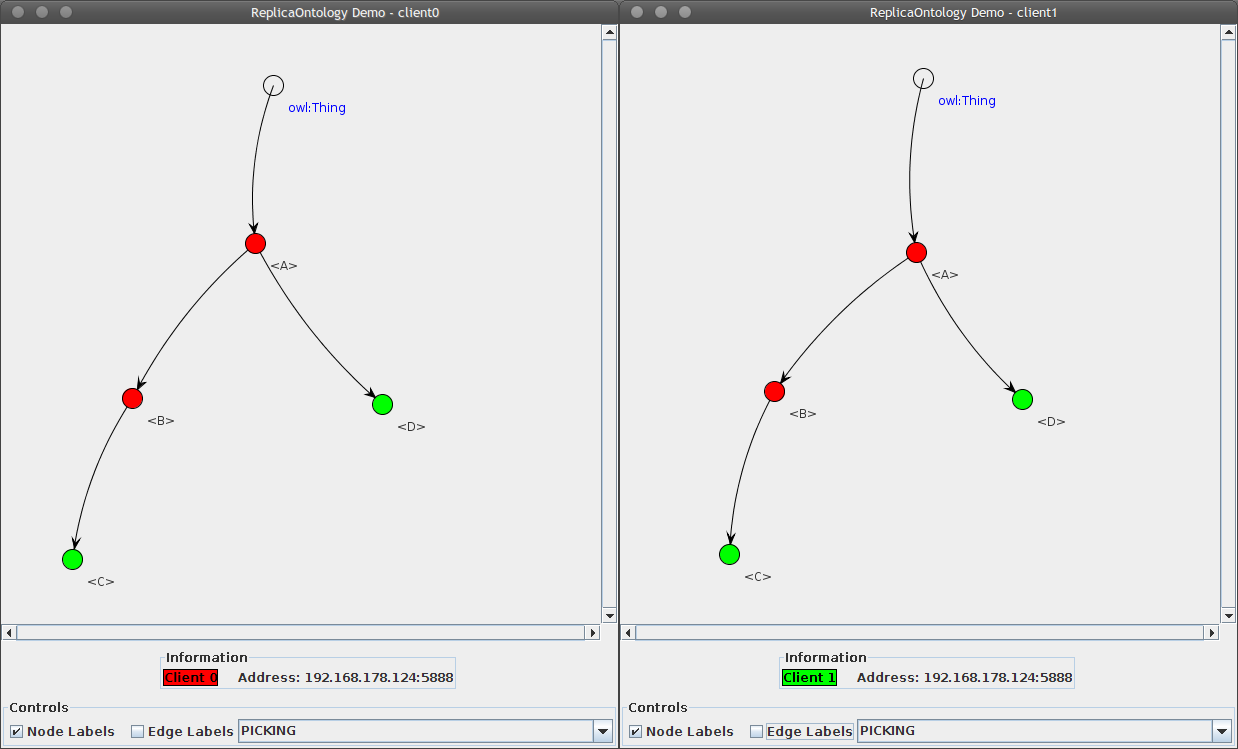
\includegraphics[width=\textwidth]{BilderFrontendImpl/demonstrator.png}
        \end{center}
        \label{fig_demo}
\end{figure}

%\begin{table}[H]
%\centering
%\footnotesize % alternativ \tiny \scriptsize \footnotesize \normalsize \large ...
%\begin{tabular}{|c|c|c|c|c|}\hline
%\bf Filename & \bf Originating project & \bf Used in bundles & \bf License & \bf Description       \\ \hline
%org.aspectj.runtime.jar  &  AspjectJ &  all &  EPL 1.0  &  AspectJ runtime     environment         \\ \hline
%org.aspectj.weaver.jar  &  AspjectJ &  all &  EPL 1.0  &  AspectJ weaver         \\ \hline
%ajde.jar  &  AspjectJ &  all &  EPL 1.0  &  AspectJ weaver     \\ \hline
%\end{tabular}
%\caption{Table of libraries used}
%\label{hd44780befehle}
%\end{table}
